\chapter{Introduction}
\label{chapter:Introduction}



% Here starts the thesis with an introduction. Please use nice latex and bibtex entries \cite{latex}. Do not spend time on formating your thesis, but on its content. 
 
\section{Motivation}
As we progress from livelihood fisheries to aquaculture industries, the global 
production and demand of fishes has drastically increased over several decades. 
According to \cite{Asche2011}, the production increased from 16 M in the 1970s to 
142 M in 2008. In these statistical figures, the amount if wild fishes has reached 
a threshold since 1980s while the farmed fishes picked up the difference in amount.
For instance, \citeauthor{LARSEN2011a} mention in \citeyearpar{LARSEN2011a} that Norway 
alone increased their production of Salmons from a few thousand in the 1980s to 
approximately 1.4 M in 2009 which constitutes around 51\% of the global supply. 
This amkes then the largest supplier of Salmons in the world \citep{Asche2011, LARSEN2011a, Liu2011}.

Other than favorable geographical and enviromental features that made Norway viable 
for this industrym technological advancement also played an important role in the 
economical cycle between demand and supply. As production increase, they reduced 
cost and as a consequence, increased the demand \cite{Asche2011}. Therefore, this cycle 
supported the growth of the industry over the years.
Since around, 80 \% of all sales of farmed fish are arranged pre-harvest, the porfit 
on the sale directly depends on the correct estimations of weight, size distribution 
and total biomass. Therefore, our project deals with remote monitoring of fishes size 
and weight distribution in aquaculture environments. Considering a large amount of fish, 
it becomes essential to develop an automated biomass estimator to constantly monitor 
the changes or growth of fishes. This system involves cameras that would detect the 
fish in a video sequence and compute the biomass distribution over a specified period 
of time.
\todo {Add description of hardware setup}

\todo { check this praragraph}
Underwater stereo-video measurement systems are used widely for counting
and measuring fish in aquaculture, fisheries and conservation management.
To determine population counts, aptial or temporal frequecies, most commonly
 using a point and click process by human operator.
Current research aims to use stereo 3d depth vision system. 
A fully automated process will requiere the detection and identification
of candidates for measerument, followed by the SNOUT to fork length measurement, 
as well as the counting and tracking of fish. This Thesis present a review and 
implementation of techniques uses for the detection, Identification, measurement, 
counting and tracking of fish in underwater image sequences, including consideration 
of the changing in body shape.
The review will analyse the most commonly used approaches, leading to an evaluation 
of techniques most likely to be a  general solution to the complete process of 
detection, measurement, counting and tracking


\section{Problem Statement}

This work is part of the project call fishscan, where the main goal is design a system for remote monitoring of fishes size and weight distribution in aquaculture environments. during this project was develop a camera rig system consist in a underwater housing with a time of flight camera with LED light source and a 2D CCD grayscale camera as is shown in the fig \ref{fig:rigsetup}.

\begin{figure}[h]
\centering
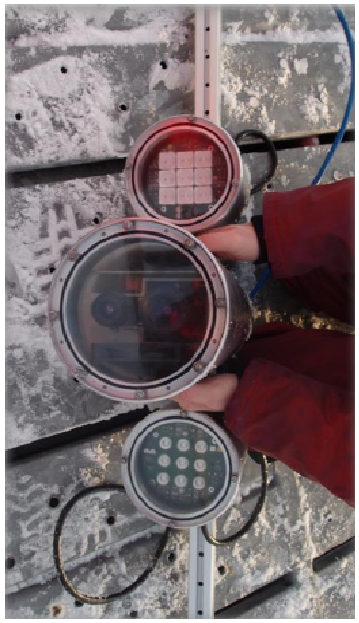
\includegraphics[scale=0.5]{rigsetup}
\caption{Rig Camera System - TOF + CCD cameras}
\label{fig:rigsetup}
\end{figure}


as the main goal of the project is compute the biomass of the fish by computing 
the volume of it, taken the concept of mass density from the physics, using the relation
between biomass and volume. Then, this problem of biomass estimation can be formulated
as a problem of volume estimation of the fish. to achieve this objective, the first 
step is the fish detection in an 2D grayscale image. followed by a backprojection 
into the TOF image where the is possible to fit a 3D model to the detected fish.
it is important to mention that the approach assume in this work is due of highly 
noisy image acquire by the range imaging camera, which was adapted to work in a 
underwater environment, but as you can see in the 3D image shown in \ref{fig:tofNoisy}


\begin{figure}[h]
\centering
\subfigure[Intensity Image TOF camera]{
	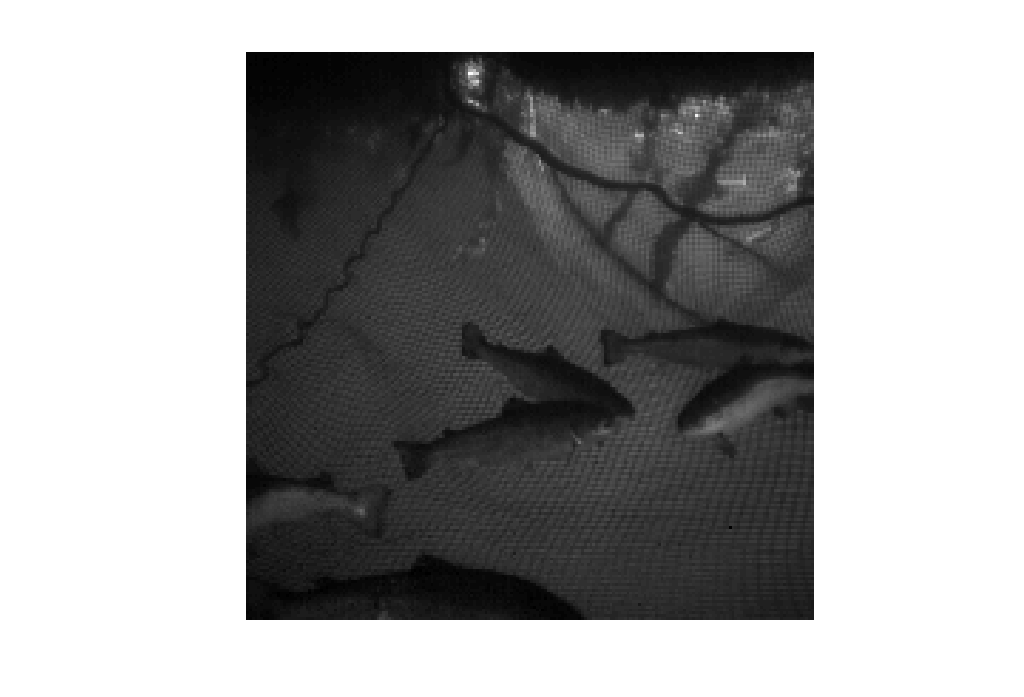
\includegraphics[scale=0.3]{tof_1}
}\subfigure[depth Image]{
	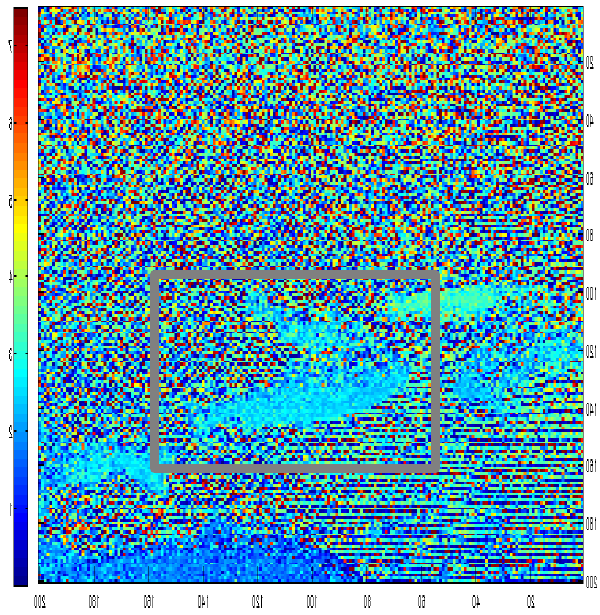
\includegraphics[scale=0.3]{tof_2}
}
% \qquad
\subfigure[3D represemtation depth image]{
	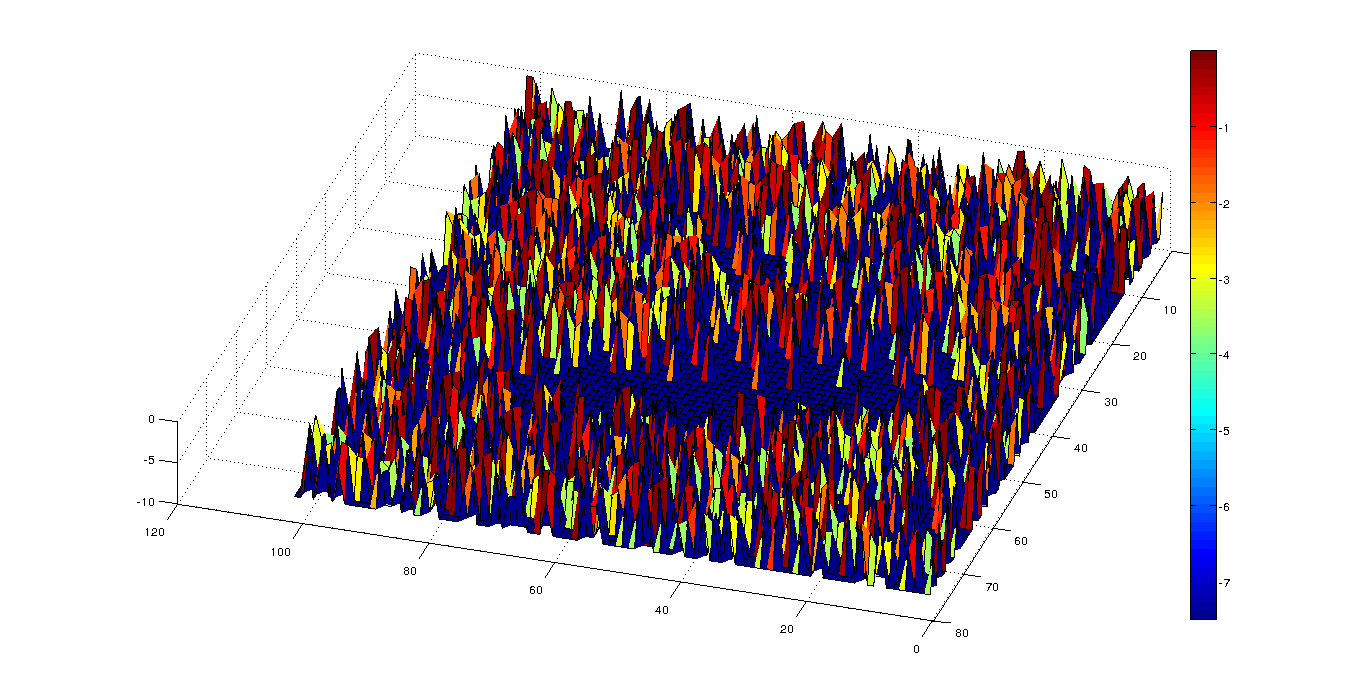
\includegraphics[scale=0.3]{tof_3}
}%
\caption{TOF camera images.}
\label{fig:tofNoisy}
\end{figure}

although, the detection using the 2D intensity image alone cannot compute the volume
of the fish because it is not depth invariant and the size is up-to-scale; This work 
will may use of the 2D intensity image as a First step, detecting the fish contour.
The pipeline depicted in \todo{ add image ref \ref{}} consist of three major steps
that are: fish detection, contour extraction, volume-biomass estimation. In this 
project, we concentrate on the first step that is fish detection and contour extraction.

At this point we need to find a algorithm for fish detection and contour extraction 
that addresses the three major challenges of our problem, These are:

\begin{enumerate}
\item \textit{Deformations}, THe algorithm must handle different motions of the
which suggests that we are dealing with a deformable (articulated) object.
\item \textit{Different Viewpoints}, As the fish move around its environment, the 
algorithm must be able to detect the fish from different perspectives.
\item \textit{Occlusions}, The algorithm must also be able to handle occlusion, 
e.g. self occlusions, occlusion from another fishes and occlusion from object in 
the environment.
\end{enumerate}
\todo { Continue from here}
The monitoring of fish for stock assessment in aquaculture,
commercial fisheries and in the assessment of the effectiveness of biodiversity 
management strategies such as Marine Protected Areas and closed area management 
is essential for the economic and environmental management of fish population,
Video based techniques for fishery independent and non-destructive sampling now 
widely accepted.
The advantages od suing stereo-video for counting the numbers of fish. measuring 
their lenght and defining the sample area have been well demostrated.
However, the time lag and cost of processing video imagery decreases the cost of 
miffectiveness and uptake of this technology. Current research aims t
	


% \section{Next Section}
% There is no need for a latex introduction since there is plenty of literature out there.
